\section{Introduction}

A microgrid is a networked group of distributed energy sources with the goal of generating, converting and storing energy. While the main power stations on central smart grid are highly connected, microgrids can operate independently or share power with the neighboring microgrid nodes \cite{farhangi2010path} on the central grid to which they are connected.

In order to take full advantage of the modularity and flexibility of microgrid technologies, smart control mechanisms are required to manage and coordinate these distributed energy systems so as to minimize the costs of energy production, conversion and storage, without jeopardizing the central smart grid stability. Augmenting microgrid with smart controls however involves addressing many problems. In this paper, we address two  problems. (i) Supply-side management problem: energy sharing among the microgrids under stochastic supply \& demand along with the optimal battery scheduling of each microgrid (ii) Demand-side management problem: efficiently scheduling the time adjustable demand from smart appliances in the smart home environments along with the normal demand. Our goal here is to reduce the energy demand and supply deficit in the long-run. We address these learning and scheduling problems by modeling them as a Markov decision process (MDP) \cite{puterman2014markov}.

\subsection{Supply-side management(SSM) problem}
Cooperative energy exchange among microgrids is a popular technique in SSM for efficient energy distribution.  Local energy sharing/exchange between microgrids has the following advantages:
(a) it can significantly reduce power wastage that would otherwise result over long distance transmission lines, and (b) it helps satisfy demand and reduce resilience on the main grid. Figure~\ref{gridmodel} shows a cooperative energy exchange model with multiple microgrids that can cater to their individual local loads. Each microgrid controls its local sub-network through its controller (labeled $\mbox{C}_1$, $\mbox{C}_2$ etc.) that mainly has access to its local state information.


\begin{figure}[thpb]
      \centering
      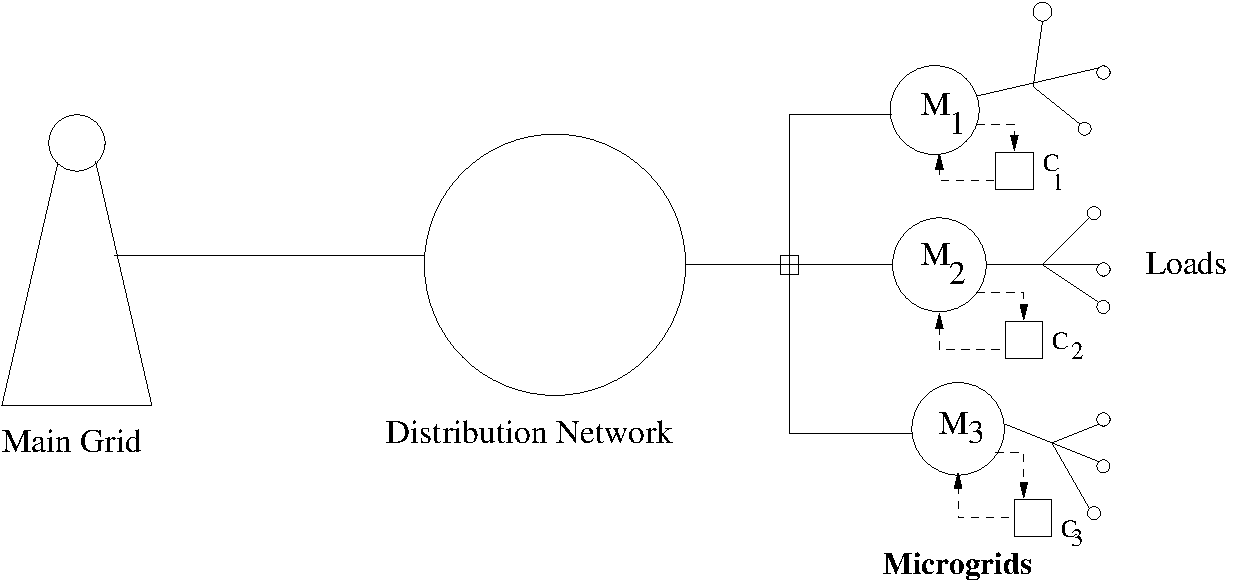
\includegraphics[scale=0.4]{powergrid2.pdf}
      \caption{Cooperative Energy Exchange Model}
      \label{gridmodel}
\end{figure}

In classical power grids, system level optimization is done based on a centralized objective function, where as microgrid network has heterogeneous nature right from the manner in which electricity is generated such as from wind turbines, solar farms and diesel generators to energy storage devices such as batteries and capacitors. Because of this heterogeneity and the fact that energy can be shared between microgrids depending on requirements, one needs to consider asynchronous distributed techniques 
%such as multi-agent reinforcement learning or game theory
to control and optimize a smart grid system connected to microgrid distribution networks.

\subsection{Demand-side management(DSM) problem}
 Load shifting is a popular technique used in DSM \cite{DTU2010}. It involves moving the consumption of load to different times within a window of an hour, or a day, etc. It doesn't lead to reduction in net quantity of energy consumed, but simply involves changing the time when the energy is consumed. While load shifting facilitates the customer in reducing the energy consumption cost, it helps the smart grid in managing the peak load.

With the increased use of the smart appliances and smart home environments, the concept of load shifting is becoming increasingly handy for the smart grid as the demand from smart appliances is time adjustable in general. One or more of these smart appliances collectively achieve some activity in the smart home environment, called as an ADL (activity of daily living). It's possible to monitor and identify the ADLs in the smart home environments \cite{GPG2016}. When an ADL is active, the smart appliances associated with that ADL are switched on to perform the activity defined by the ADL thus adding load on the smart grid. With the help of the smart home technology, it's possible to find the amount of load each ADL puts on the grid, and also the allowed time window during which the ADL would perform the activity (e.g., washing machine running for an hour to clean the cloths anytime between 3PM to 6PM). If the time window for the ADL lets the smart grid have more than one possible way of scheduling the load, it's considered as flexible ADL. On the other hand, if the time window for the ADL lets the smart grid have exactly one possible way of scheduling the load, it's considered as non-flexible ADL (e.g., washing machine running for an hour to clean the cloths anytime between 3PM to 4PM, is not flexible since there is only one option of switching on the washing machine at 3PM). Thus the demand from the flexible ADLs need not be met at a fixed time period, instead could be met at any time period within a flexible time window. With the help of the advanced metering infrastructure (AMI) that provides a two-way communication between the utility and customers, it's possible to take the decision of when to schedule the ADL demand at the smart grid and convey the same to the customer's smart meter.    

There is other regular demand that needs to be met at fixed time periods, apart from the zero or more ADL related demand associated with any customer. This regular demand along with the zero or more non-flexible ADL demand of a smart home is considered to be non-ADL demand for the rest of the paper. Similarly, the demand due to zero or more flexible ADLs of the smart home is considered to be ADL demand.

\textbf{Related work :} There is prior art around scheduling the ADL-demand using the load shifting technique for handling the peak load scenarios \cite{CL2014}. However, they precisely know the supply profile while doing such a scheduling of the ADL-demand. In this paper, we propose scheduling of ADL-demand using the load shifting technique with uncertainty in the supply profile generated (e.g., renewable energy sources like solar or wind being the primary sources of power generation).
 \cite{saad2012game} provides a survey on game theoretic approaches for microgrids where both cooperative energy sharing models as well as non-cooperative game models for distributed control of microgrids are examined when the system model is known (i.e., demand \& supply profile are known ahead). Since  models for energy dynamics are very unreliable \cite{zamora2010controls}, one has to use model-free algorithms to address these problems.  Because of their model-free nature, reinforcement learning \cite{sutton1998reinforcement} approaches that are primarily data-driven control techniques are playing a significant role in these problems.

In \cite{zifadistributed}, distributed reinforcement learning algorithm for coordinated energy sharing and voltage restoration in a islanded DC microgrid is proposed. In \cite{leo2014reinforcement}, reinforcement learning algorithm for optimal battery scheduling under the dynamic load environment and solar power is proposed with the goal of  reducing  energy consumption from the main grid. In this paper, we  consider the coordinated energy sharing among the grid connected microgrids with optimal battery scheduling problem when stochastic supply and adjustable stochastic demand is available.

\textbf{Our contributions :}
\begin{inparaenum}[\bfseries (i)]
We summarize our contributions as follows :\\
\item To the best of our knowledge, we are the first one to integrate both the Demand-side and Supply-side management problems  in a single Markov decision process framework. We used reinforcement learning algorithms which do not require knowledge of the underlying model to address these problems. Our algorithms are easy to implement and also scalable.\\
\item The Optimal scheduling of ADL demand at microgrid level, where both the demand and power generation is stochastic is first time introduced through this work. \\    
\end{inparaenum}

The rest of the paper is organized as follows. In the section \ref{sec:model}, we discuss in detail about the problem formulation using MDP framework. We present  in section \ref{sec:algo} about our Q-learning algorithm. In section \ref{sec:experiments}, we present simulation experiments along with other algorithms for comparison. Finally in section \ref{sec:conclusion}, we provide the concluding remarks.